\section{换基与最优性判别}
\label{sec:simplex-basis-exchange}

手里已经有一个可行的顶点时，怎样判断它是不是最优；如果不是，下一步该走到哪里？

\paragraph{一个资源配置问题}
工厂生产两种产品，产量分别记为$x_1,x_2$，单位利润分别是$4$和$5$。原料有$8$单位，工时有$10$单位，产品二还要占用一台专用设备，设备最多加工$3$单位。两种产品对原料和工时的消耗写在下面的约束里，于是问题是
\begin{equation}
 \begin{aligned}
 \max_{x_1,x_2}\quad & 4x_1+5x_2\\
 \text{s.t.}\quad & x_1+2x_2\leq 8,\\
 & 2x_1+x_2\leq 10,\\
 & x_2\leq 3,\qquad x_1,x_2\geq 0.
 \end{aligned}
 \label{eq:simplex-resource-problem}
\end{equation}
图~\ref{fig:simplex-resource-vertices}画出它的可行域，这是一个有五个顶点的多边形。虚线是利润的等值线，沿箭头方向利润增大，最后离开多边形的那个点就是最优解。

\begin{BookInlineFigure}
 \centering
 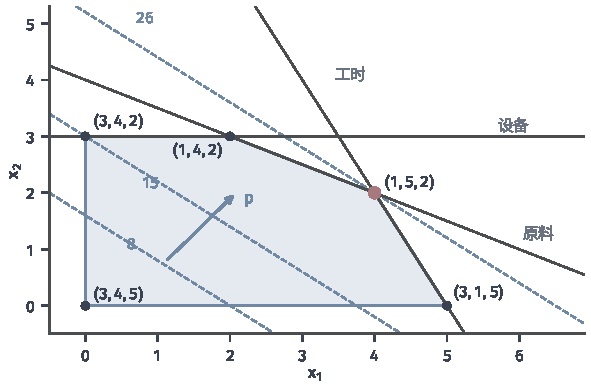
\includegraphics[width=100mm]{figures/05-optimization/01-linear-programming/matplotlib/simplex-resource-vertices/figure.pdf}
 \caption{资源配置问题~\eqref{eq:simplex-resource-problem}的可行域（浅蓝）。三条深灰线分别是原料、工时和设备约束的边界，蓝色虚线是利润$4x_1+5x_2$取$8,15,26$的等值线，箭头$\bm{p}=(4,5)$指向利润增大的方向。每个顶点旁的三元组是它对应的基，红点是最优顶点$(4,2)$。}
 \label{fig:simplex-resource-vertices}
\end{BookInlineFigure}

二维时用眼睛就能找到最优点，但变量一多就画不出来，需要把“在顶点上看哪条边更好”翻译成矩阵运算。先引入松弛变量$x_3,x_4,x_5\geq0$，分别表示没有用完的原料、工时和设备能力，并把最大化改写成最小化，得到第~\ref{chap:linear-programming}章的标准型
\begin{equation}
 \min_{\bm{x}}\ \bm{c}^\top\bm{x}\quad\text{s.t.}\quad \bm{A}\bm{x}=\bm{b},\quad \bm{x}\geq\bm{0},
 \label{eq:simplex-standard-form}
\end{equation}
其中$\bm{A}\in\mathbb{R}^{m\times n}$满行秩，第$j$列记为$\bm{a}_j=\bm{A}_{:,j}$。本例中$m=3$，$n=5$，数据是
\begin{equation}
 \bm{A}=\begin{bmatrix}1&2&1&0&0\\2&1&0&1&0\\0&1&0&0&1\end{bmatrix},\quad
 \bm{b}=\begin{bmatrix}8\\10\\3\end{bmatrix},\quad
 \bm{c}=\begin{bmatrix}-4\\-5\\0\\0\\0\end{bmatrix}.
 \label{eq:simplex-resource-data}
\end{equation}
最小化的目标值$f=\bm{c}^\top\bm{x}$是负的利润，所以下文中$f$越小，利润越大。

\paragraph{基与顶点}
第~\ref{chap:linear-programming}章已经建立了下面要用的事实。取$m$个下标组成有序元组$B$，使基矩阵$\bm{A}_B$可逆，这样的$B$称为基，其余下标组成$N$。令非基分量为零，基分量为
\[
 \bm{x}_B=\bm{A}_B^{-1}\bm{b},\qquad \bm{x}_N=\bm{0},
\]
就得到一个基本解。$\bm{x}_B\geq\bm{0}$时它是基本可行解，也就是可行域的极点；问题可行且最优值有限时，最优解可以在基本可行解中取得。所以只需在基之间搜索。下标属于$B$的变量称为\term{基变量}（basic variable），其余的称为\term{非基变量}（nonbasic variable）。

以顶点$(4,2)$为例，此时原料和工时恰好用完，即$x_3=x_4=0$，而设备还余$x_5=1$。非基变量是$x_3,x_4$，基变量是$x_1,x_5,x_2$，我们把基写成$B=(1,5,2)$。元组的顺序用来对应$\bm{x}_B$的分量，换基时新变量占据被换出变量的位置，顺序因此保持稳定。

\paragraph{主要思想：用非基变量表示一切}
站在一个顶点上，我们想知道沿每条边走会怎样。非基变量恰好提供了一组局部坐标：它们此刻都是零，让其中一个变大，就是离开顶点走上一条边。因此要把基变量和目标都写成非基变量的函数。

把$\bm{A}\bm{x}=\bm{b}$按基和非基拆开，得到$\bm{A}_B\bm{x}_B+\bm{A}_N\bm{x}_N=\bm{b}$。两边左乘$\bm{A}_B^{-1}$，每个满足等式约束的点都有
\begin{equation}
 \bm{x}_B=\bm{A}_B^{-1}\bm{b}-\bm{A}_B^{-1}\bm{A}_N\bm{x}_N.
 \label{eq:simplex-basic-form}
\end{equation}
代入目标后，整理非基变量的系数：
\[
 \bm{c}^\top\bm{x}
 =\bm{c}_B^\top\bm{x}_B+\bm{c}_N^\top\bm{x}_N
 =\bm{c}_B^\top\bm{A}_B^{-1}\bm{b}
 +\bigl(\bm{c}_N^\top-\bm{c}_B^\top\bm{A}_B^{-1}\bm{A}_N\bigr)\bm{x}_N.
\]

系数里反复出现$\bm{c}_B^\top\bm{A}_B^{-1}$，把它单独命名。记
\begin{equation}
 \bm{y}=\bm{A}_B^{-\top}\bm{c}_B,
 \qquad
 s_j=c_j-\bm{a}_j^\top\bm{y}\quad(j=1,\ldots,n),
 \label{eq:simplex-reduced-cost}
\end{equation}
其中$\bm{y}\in\mathbb{R}^m$称为这个基的对偶候选，$s_j$称为$x_j$的\term{约化成本}（reduced cost）。对基变量，$\bm{A}_B^\top\bm{y}=\bm{c}_B$正好说明$s_j=0$（$j\in B$）。于是每个满足等式约束的点都有
\begin{equation}
 \bm{c}^\top\bm{x}=\bm{b}^\top\bm{y}+\sum_{j\in N}s_jx_j.
 \label{eq:simplex-objective-form}
\end{equation}

这个式子是本章的出发点。第一项是当前顶点的目标值，第二项说明：让非基变量$x_j$从零增加一个单位，目标改变$s_j$。可以这样理解这些量：$y_i$是这个基给第$i$种资源定的内部单价，$\bm{a}_j^\top\bm{y}$是生产一单位$x_j$所耗资源按内部单价折算的总价，$s_j$是$x_j$的真实成本减去这个折算价。$s_j<0$表示真实成本比折算价低，做这件事划算。

这组记号和第~\ref{chap:linear-programming}章的对偶是同一套。对偶问题要求$\bm{A}^\top\bm{y}+\bm{s}=\bm{c}$且$\bm{s}\geq\bm{0}$，而式~\eqref{eq:simplex-reduced-cost}总满足前一半，只差$\bm{s}\geq\bm{0}$。“候选”二字指的就是这一点：等式已经成立，符号条件还要检查。

\begin{theorem}[最优性判别]
 \label{thm:simplex-optimality}
 设$B$是可行基，基本可行解为$\bar{\bm{x}}$，$\bm{y},\bm{s}$由式~\eqref{eq:simplex-reduced-cost}给出。若
 \begin{equation}
  s_j\geq 0\quad\text{对所有 }j\in N\text{ 成立},
  \label{eq:simplex-optimality-condition}
 \end{equation}
 则$\bar{\bm{x}}$是标准型~\eqref{eq:simplex-standard-form}的全局最优解，$(\bm{y},\bm{s})$是对偶最优解，两者目标值相等。
\end{theorem}

\begin{proof}
 任取可行点$\bm{x}$。它满足$\bm{A}\bm{x}=\bm{b}$，所以式~\eqref{eq:simplex-objective-form}对它成立。又因$\bm{x}_N\geq\bm{0}$且$s_j\geq0$，右端第二项非负，于是
 \[
  \bm{c}^\top\bm{x}\geq\bm{b}^\top\bm{y}.
 \]
 另一方面$\bar{\bm{x}}_N=\bm{0}$，式~\eqref{eq:simplex-objective-form}给出$\bm{c}^\top\bar{\bm{x}}=\bm{b}^\top\bm{y}$。所以$\bar{\bm{x}}$的目标值不大于任何可行点的目标值。条件~\eqref{eq:simplex-optimality-condition}连同基变量的$s_j=0$说明$(\bm{y},\bm{s})$对偶可行，它的对偶目标$\bm{b}^\top\bm{y}$等于原始目标，由弱对偶知它是对偶最优解。
\end{proof}

判别只看当前顶点的约化成本，结论却是全局的，原因在于式~\eqref{eq:simplex-objective-form}对所有满足等式的点都成立，不是局部近似。约化成本全部非负，就等于对偶可行，$\bm{y}$就是第~\ref{chap:linear-programming}章说的下界证书。

定理的方向只有一个：非负是最优的充分条件。某个$s_j<0$时，当前顶点是否一定不是最优，要看沿这条边能否真的走出去，这正是下面要讨论的。

\paragraph{主要思想：沿一条边走到下一个顶点}
设$s_q<0$，$q\in N$，我们让$x_q$增大，其余非基变量保持为零。记增大的幅度为$\alpha\geq0$，由式~\eqref{eq:simplex-basic-form}，基变量随之按下式变化：
\begin{equation}
 \bm{x}_B(\alpha)=\bar{\bm{x}}_B-\alpha\bm{u},\qquad \bm{u}=\bm{A}_B^{-1}\bm{a}_q.
 \label{eq:simplex-direction}
\end{equation}
$\bm{u}$的含义很具体：$u_i$是$x_q$每增加一单位时，位于第$i$个位置的基变量要减少的量。用整个向量来写，移动方向$\bm{d}\in\mathbb{R}^n$满足$d_q=1$，$\bm{d}_B=-\bm{u}$，其余分量为零。

沿这个方向走，等式约束不被破坏，目标按$s_q$下降。两件事都可以直接验算：
\[
 \bm{A}\bm{d}=\bm{a}_q-\bm{A}_B\bm{u}=\bm{0},
 \qquad
 \bm{c}^\top\bm{d}=c_q-\bm{c}_B^\top\bm{A}_B^{-1}\bm{a}_q=s_q.
\]

图~\ref{fig:simplex-edge-rates}在顶点$(2,3)$上画出了这两种可能。这个顶点的基是$(1,4,2)$，$x_3,x_5$非基。让$x_3$增大，点沿设备约束的边向左移动，目标以速率$s_3=4$变差；让$x_5$增大，点沿原料约束的边向右下移动，目标以速率$s_5=-3$变好。

\begin{BookInlineFigure}
 \centering
 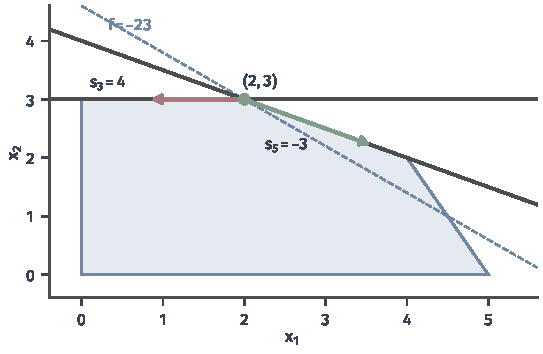
\includegraphics[width=92mm]{figures/05-optimization/01-linear-programming/matplotlib/simplex-edge-rates/figure.pdf}
 \caption{顶点$(2,3)$处的两条边。深灰粗线是在此活动的设备和原料约束，蓝色虚线是过该点的等值线$f=-23$。红色箭头是$x_3$增大的方向，走上去$f$每单位增加$4$；绿色箭头是$x_5$增大的方向，走上去$f$每单位减少$3$，它越过等值线进入利润更高的一侧。}
 \label{fig:simplex-edge-rates}
\end{BookInlineFigure}

能走多远由基变量的非负性决定。$u_i\leq0$的基变量不会减小，不构成限制；$u_i>0$的基变量在$\alpha=\bar{x}_{B(i)}/u_i$时降到零，其中$B(i)$是基中第$i$个下标。最先降到零的那个变量决定步长：
\begin{equation}
 \alpha^\star=\min_{i:\,u_i>0}\frac{\bar{x}_{B(i)}}{u_i}.
 \label{eq:simplex-ratio-test}
\end{equation}
这称为\term{比值检验}（ratio test）。像预算线一样，每种资源各自算出“还够做多少”，能做的量由最紧的那一种决定。图~\ref{fig:simplex-ratio-test}把基变量画成$\alpha$的直线，第一条碰到零的直线给出步长。

\begin{BookInlineFigure}
 \centering
 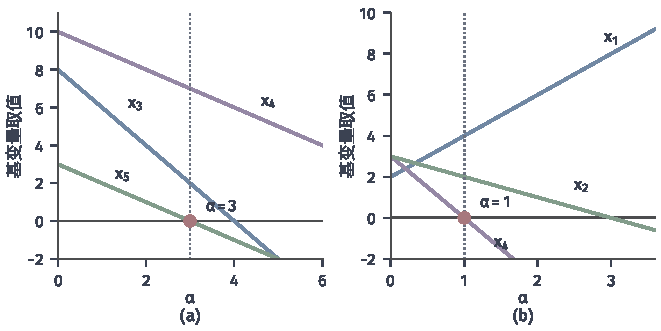
\includegraphics[width=112mm]{figures/05-optimization/01-linear-programming/matplotlib/simplex-ratio-test/figure.pdf}
 \caption{比值检验的两个实例，三条直线是基变量随步长$\alpha$的变化，红点是最先降到零的位置。(a)~入基变量$x_2$，基$(3,4,5)$，$x_5$先到零，$\alpha^\star=3$。(b)~入基变量$x_5$，基$(1,4,2)$，$x_1$随$\alpha$增大而增大，不起限制作用，$x_4$先到零，$\alpha^\star=1$。}
 \label{fig:simplex-ratio-test}
\end{BookInlineFigure}

设最小值在位置$r$取到，$p=B(r)$。走到$\alpha^\star$后$x_p=0$，$x_q=\alpha^\star$，于是把$p$从基中换出、$q$换入。$x_q$称为\term{入基变量}（entering variable），$x_p$称为\term{出基变量}（leaving variable），这一次替换称为\term{换基}（pivot）。下面的引理保证替换后仍是一个可行基。

\begin{lemma}[换基的合法性]
 \label{lem:simplex-pivot}
 设$s_q<0$，$\bm{u}$由式~\eqref{eq:simplex-direction}给出且$\bm{u}$至少有一个正分量，$r$在式~\eqref{eq:simplex-ratio-test}中取到最小值。把$B$的第$r$个下标换成$q$，得到的$B'$仍是基，$\bar{\bm{x}}+\alpha^\star\bm{d}$是它的基本可行解，目标值为
 \begin{equation}
  \bm{c}^\top\bar{\bm{x}}+\alpha^\star s_q.
  \label{eq:simplex-objective-update}
 \end{equation}
\end{lemma}

\begin{proof}
 先证$\bm{A}_{B'}$可逆。由$\bm{A}_B\bm{u}=\bm{a}_q$，有$\bm{a}_q=\sum_iu_i\bm{a}_{B(i)}$，其中$\bm{a}_{B(r)}$的系数$u_r>0$。若$\bm{A}_{B'}$的列线性相关，由于其余$m-1$列线性无关，$\bm{a}_q$就能只用这$m-1$列表示，这与$\bm{a}_q$在基$\bm{A}_B$下表示的唯一性及$u_r\neq0$矛盾。

 再看新点。由$\bm{A}\bm{d}=\bm{0}$，等式约束保持成立。$\alpha^\star$的取法使所有基变量非负，$x_q=\alpha^\star\geq0$。新点在位置$p$和$N\setminus\{q\}$上的分量都是零，也就是$B'$之外的分量都是零，所以它是$B'$的基本可行解。目标值由$\bm{c}^\top\bm{d}=s_q$得到。
\end{proof}

$\alpha^\star>0$时，目标严格下降，点从一个顶点沿边走到了相邻顶点。这就是单纯形法的全部几何内容。

\needspace{6\baselineskip}
\paragraph{变量}
下面用工厂的例子走完整个过程。计算中出现的量及其形状如下。
\begin{itemize}
 \item $B^{(t)}$：第$t$轮的基，含$m$个下标的有序元组；$N^{(t)}$是其余$n-m$个下标。
 \item $\bm{x}_B^{(t)}\in\mathbb{R}^m$：基变量的取值，非基变量都是零。
 \item $\bm{y}^{(t)}\in\mathbb{R}^m$：对偶候选。
 \item $s_j^{(t)}$：非基变量的约化成本。
 \item $q^{(t)}$：入基下标；$\bm{u}^{(t)}\in\mathbb{R}^m$：入基列在当前基下的表示。
 \item $\alpha^{(t)}\geq0$：步长；$r^{(t)}$：出基位置，$p^{(t)}=B^{(t)}(r^{(t)})$是出基下标。
\end{itemize}

\paragraph{初始化}
需要一个可行基$B^{(0)}$。当$\bm{b}\geq\bm{0}$且每个约束都带松弛变量时，取全部松弛变量为基即可，此时$\bm{A}_B=\bm{I}$。其他情形在第~\ref{sec:simplex-initial-basis}节处理。例中
\[
 B^{(0)}=(3,4,5),\qquad \bm{A}_{B^{(0)}}=\bm{I},\qquad \bm{x}_B^{(0)}=\begin{bmatrix}8\\10\\3\end{bmatrix}.
\]
对应顶点$(0,0)$，什么都不生产，$f=0$。

\needspace{6\baselineskip}
\paragraph{每轮更新}
第$t$轮依次做下面几步。步骤后的“例中”是第$0$轮的数据，其余各轮随后列出。
\begin{enumerate}

 \item 计算对偶候选。由式~\eqref{eq:simplex-reduced-cost}，
 \[
  \bm{y}^{(t)}=\bigl(\bm{A}_{B^{(t)}}\bigr)^{-\top}\bm{c}_{B^{(t)}}.
 \]
 例中$\bm{c}_B=\bm{0}$，所以
 \[
  \bm{y}^{(0)}=(0,0,0)^\top.
 \]

 \item 定价，即对每个非基下标计算约化成本$s_j^{(t)}=c_j-\bm{a}_j^\top\bm{y}^{(t)}$。例中
 \[
  s_1^{(0)}=-4,\qquad s_2^{(0)}=-5.
 \]

 \item 判别。若所有$s_j^{(t)}\geq0$，停止，当前解最优。否则选一个$s_q^{(t)}<0$的下标$q=q^{(t)}$入基。本节取约化成本最负的下标，称为\term{Dantzig规则}（Dantzig's rule），并列时取下标最小者。例中$s_2$最负，所以
 \[
  q^{(0)}=2.
 \]

 \item 计算入基列的表示。由式~\eqref{eq:simplex-direction}，
 \[
  \bm{u}^{(t)}=\bigl(\bm{A}_{B^{(t)}}\bigr)^{-1}\bm{a}_q.
 \]
 若$\bm{u}^{(t)}\leq\bm{0}$，停止，问题无界。例中
 \[
  \bm{u}^{(0)}=\bm{a}_2=(2,1,1)^\top.
 \]

 \item 比值检验。由式~\eqref{eq:simplex-ratio-test}求$\alpha^{(t)}$和出基位置$r^{(t)}$，并列时本节取下标最小的基变量。例中三个比值是
 \[
  \frac{x_3}{u_1}=\frac{8}{2}=4,\qquad
  \frac{x_4}{u_2}=\frac{10}{1}=10,\qquad
  \frac{x_5}{u_3}=\frac{3}{1}=3,
 \]
 所以
 \[
  \alpha^{(0)}=3,\qquad r^{(0)}=3,\qquad p^{(0)}=5.
 \]

 \item 更新基和基变量。除第$r$个位置外，
 \begin{equation}
  \bm{x}_B^{(t+1)}=\bm{x}_B^{(t)}-\alpha^{(t)}\bm{u}^{(t)},
  \label{eq:simplex-primal-update}
 \end{equation}
 第$r$个位置改放$x_q=\alpha^{(t)}$，并把$B^{(t)}$的第$r$个下标换成$q$。例中
 \[
  B^{(1)}=(3,4,2),\qquad \bm{x}_B^{(1)}=\begin{bmatrix}8-3\cdot2\\10-3\cdot1\\3\end{bmatrix}=\begin{bmatrix}2\\7\\3\end{bmatrix}.
 \]
 目标值由式~\eqref{eq:simplex-objective-update}变为$0+3\cdot(-5)=-15$，点走到$(0,3)$。
\end{enumerate}

例中第$1$轮的基矩阵是
\[
 \bm{A}_{B^{(1)}}=\begin{bmatrix}1&0&2\\0&1&1\\0&0&1\end{bmatrix}.
\]
解$\bm{A}_B^\top\bm{y}=\bm{c}_B$，其中$\bm{c}_B=(0,0,-5)^\top$，再计算两个非基变量的约化成本：
\[
 \bm{y}^{(1)}=(0,0,-5)^\top,\qquad s_1^{(1)}=-4,\qquad s_5^{(1)}=5.
\]
只有$s_1<0$，所以$x_1$入基。它的表示和两个有效比值为
\[
 \bm{u}^{(1)}=(1,2,0)^\top,\qquad
 \frac{x_3}{u_1}=\frac{2}{1}=2,\qquad
 \frac{x_4}{u_2}=\frac{7}{2}.
\]
第三个分量$u_3=0$，产品一不占专用设备，$x_2$不受影响。于是$\alpha^{(1)}=2$，$x_3$出基，更新后
\[
 B^{(2)}=(1,4,2),\qquad \bm{x}_B^{(2)}=\begin{bmatrix}2\\7-2\cdot2\\3\end{bmatrix}=\begin{bmatrix}2\\3\\3\end{bmatrix}.
\]
目标值变为$-15+2\cdot(-4)=-23$，点走到$(2,3)$。

例中第$2$轮的基矩阵和对偶候选是
\[
 \bm{A}_{B^{(2)}}=\begin{bmatrix}1&0&2\\2&1&1\\0&0&1\end{bmatrix},\qquad
 \bm{c}_B=\begin{bmatrix}-4\\0\\-5\end{bmatrix},\qquad
 \bm{y}^{(2)}=\begin{bmatrix}-4\\0\\3\end{bmatrix}.
\]
非基变量$x_3,x_5$的约化成本为
\[
 s_3^{(2)}=0-(-4)=4,\qquad s_5^{(2)}=0-3=-3.
\]
这里出现了一个值得留意的现象：$x_5$是设备的余量，让它入基意味着故意不用满设备。$s_5<0$说明把设备让出一些，腾出的原料拿去做产品一更赚钱。$x_5$入基，表示向量和比值为
\[
 \bm{u}^{(2)}=(-2,3,1)^\top,\qquad
 \frac{x_4}{u_2}=\frac{3}{3}=1,\qquad
 \frac{x_2}{u_3}=\frac{3}{1}=3.
\]
$u_1=-2<0$表示$x_1$会增大，不参与比较。于是$\alpha^{(2)}=1$，$x_4$出基，按式~\eqref{eq:simplex-primal-update}更新：
\[
 B^{(3)}=(1,5,2),\qquad
 \bm{x}_B^{(3)}=\begin{bmatrix}2+2\\1\\3-1\end{bmatrix}=\begin{bmatrix}4\\1\\2\end{bmatrix}.
\]
目标值变为$-23+1\cdot(-3)=-26$，点走到$(4,2)$。

例中第$3$轮的基矩阵和对偶候选是
\[
 \bm{A}_{B^{(3)}}=\begin{bmatrix}1&0&2\\2&0&1\\0&1&1\end{bmatrix},\qquad
 \bm{c}_B=\begin{bmatrix}-4\\0\\-5\end{bmatrix},\qquad
 \bm{y}^{(3)}=\begin{bmatrix}-2\\-1\\0\end{bmatrix}.
\]
非基变量$x_3,x_4$的约化成本为
\[
 s_3^{(3)}=0-(-2)=2,\qquad s_4^{(3)}=0-(-1)=1.
\]
两者都非负，算法停止。表~\ref{tab:simplex-resource-rounds}汇总了四轮的数据。

\begin{BookInlineTable}
 \centering
 \begin{tabular}{cccccc}
  \toprule
  $t$ & $B^{(t)}$ & $(x_1,x_2)$ & $f$ & $\bm{y}^{(t)}$ & 入基／出基\\
  \midrule
  $0$ & $(3,4,5)$ & $(0,0)$ & $0$ & $(0,0,0)$ & $x_2$／$x_5$\\
  $1$ & $(3,4,2)$ & $(0,3)$ & $-15$ & $(0,0,-5)$ & $x_1$／$x_3$\\
  $2$ & $(1,4,2)$ & $(2,3)$ & $-23$ & $(-4,0,3)$ & $x_5$／$x_4$\\
  $3$ & $(1,5,2)$ & $(4,2)$ & $-26$ & $(-2,-1,0)$ & 停止\\
  \bottomrule
 \end{tabular}
 \caption{资源配置问题在Dantzig规则下的各轮数据。}
 \label{tab:simplex-resource-rounds}
\end{BookInlineTable}

\paragraph{最终得到}
算法结束时得到最优基$B^\star=(1,5,2)$和最优解
\begin{equation}
 \bm{x}^\star=(4,2,0,0,1)^\top,\qquad p^\star=-26,
 \label{eq:simplex-resource-solution}
\end{equation}
即产品一做$4$、产品二做$2$，利润$26$，原料和工时用完，设备余$1$。同时得到对偶最优解
\begin{equation}
 \bm{y}^\star=(-2,-1,0)^\top,\qquad \bm{s}^\star=(0,0,2,1,0)^\top.
 \label{eq:simplex-resource-dual}
\end{equation}
证书可以当场核对：一方面$\bm{b}^\top\bm{y}^\star=-16-10=-26=p^\star$，另一方面$(\bm{x}^\star)^\top\bm{s}^\star=0$，互补松弛成立。

几何上，最优性说的是目标方向落在活动约束法向量张成的锥里。把最大化写回去，利润向量恰好是原料和工时两个法向量的非负组合：
\[
 \begin{bmatrix}4\\5\end{bmatrix}=2\begin{bmatrix}1\\2\end{bmatrix}+1\begin{bmatrix}2\\1\end{bmatrix}.
\]
图~\ref{fig:simplex-optimal-cone}画的就是这个分解，组合系数$2,1$正是$-\bm{y}^\star$的前两个分量。

\begin{BookInlineFigure}
 \centering
 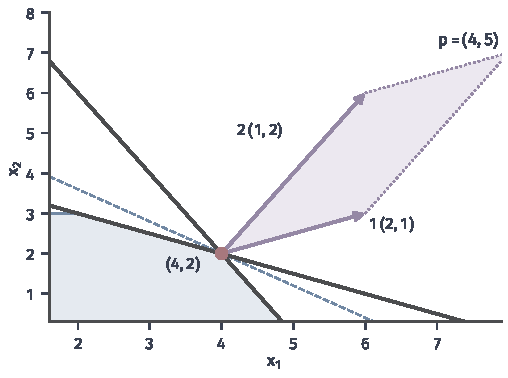
\includegraphics[width=86mm]{figures/05-optimization/01-linear-programming/matplotlib/simplex-optimal-cone/figure.pdf}
 \caption{最优顶点$(4,2)$处的对偶证书。深灰粗线是两条活动约束，紫色箭头是它们的法向量按系数$2$和$1$缩放后的结果，蓝色箭头是利润向量$\bm{p}$，它是紫色平行四边形的对角线，因此落在两个法向量张成的锥内。蓝色虚线是过该点的等值线。}
 \label{fig:simplex-optimal-cone}
\end{BookInlineFigure}

\paragraph{换基规则影响路径，不影响结论}
Dantzig规则只看单位变化率，不看能走多远。图~\ref{fig:simplex-vertex-paths}对比了同一问题上的两条路径：Dantzig规则先选利润系数大的$x_2$，走了三步；若总选下标最小的负约化成本，则先选$x_1$，经$(5,0)$两步到达。两条路径终点相同，因为最优性判别不依赖路径。这个例子不能说明后一种规则更好，它只说明步数取决于规则与问题的搭配。

\begin{BookInlineFigure}
 \centering
 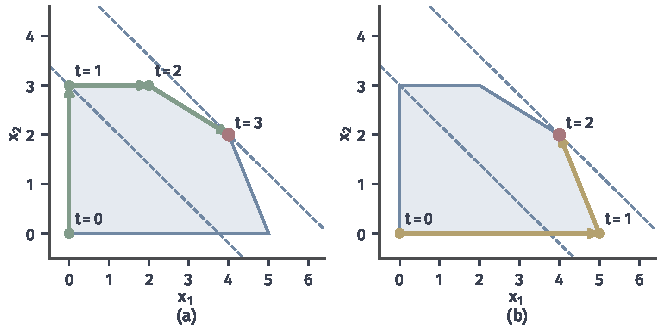
\includegraphics[width=112mm]{figures/05-optimization/01-linear-programming/matplotlib/simplex-vertex-paths/figure.pdf}
 \caption{同一问题上的两条换基路径，蓝色虚线是利润$15$和$26$的等值线，红点是最优解。(a)~Dantzig规则（绿色），经$(0,3)$和$(2,3)$共三次换基。(b)~总选下标最小的负约化成本（黄色），经$(5,0)$共两次换基。}
 \label{fig:simplex-vertex-paths}
\end{BookInlineFigure}

\paragraph{没有出基变量：无界证书}
比值检验可能找不到任何限制。此时$\bm{u}\leq\bm{0}$，对一切$\alpha\geq0$，$\bar{\bm{x}}+\alpha\bm{d}$都可行，目标按$\alpha s_q$趋于$-\infty$。这个$\bar{\bm{x}}$和$\bm{d}$合在一起就是问题无下界的证据：
\begin{equation}
 \bm{A}\bm{d}=\bm{0},\qquad \bm{d}\geq\bm{0},\qquad \bm{c}^\top\bm{d}=s_q<0.
 \label{eq:simplex-unbounded-certificate}
\end{equation}

\begin{example}[无界问题]
 \label{ex:simplex-unbounded}
 考虑最大化$x_1+x_2$，约束为$x_1-x_2\leq2$，$-x_1+x_2\leq1$，$x_1,x_2\geq0$。加松弛变量$x_3,x_4$，从$B=(3,4)$出发，约化成本是$s_1=s_2=-1$，取$x_1$入基。比值检验给出$x_3$出基，$\alpha=2$，点到达$(2,0)$。

 第二轮$B=(1,4)$，对偶候选和约化成本为
 \[
  \bm{y}=(-1,0)^\top,\qquad s_2=-2,\qquad s_3=1.
 \]
 $x_2$入基，它的表示是
 \[
  \bm{u}=(-1,0)^\top\leq\bm{0}.
 \]
 没有基变量会减小，比值检验无从进行。按式~\eqref{eq:simplex-unbounded-certificate}得到无界方向$\bm{d}=(1,1,0,0)^\top$，沿它每走一单位，目标减少$2$。
\end{example}

图~\ref{fig:simplex-unbounded}中可行域是一条向右上方延伸的带子，红色射线在带子里一直走不出去，而利润不断增大。

\begin{BookInlineFigure}
 \centering
 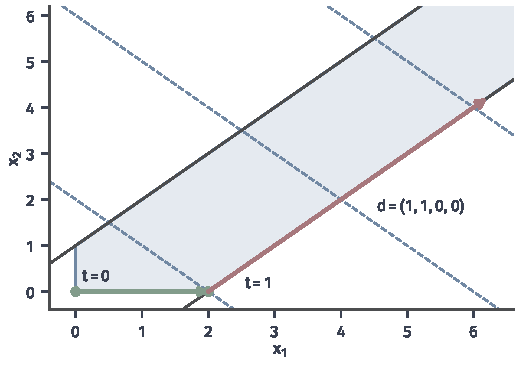
\includegraphics[width=88mm]{figures/05-optimization/01-linear-programming/matplotlib/simplex-unbounded/figure.pdf}
 \caption{例~\ref{ex:simplex-unbounded}的无界可行域（浅蓝，向右上方无限延伸）。绿色是一次换基，从$(0,0)$到$(2,0)$；红色射线是无界方向$\bm{d}$，蓝色虚线是利润$2,6,10$的等值线，射线不断穿过利润更高的等值线。}
 \label{fig:simplex-unbounded}
\end{BookInlineFigure}

\paragraph{走不动的换基}
还有一种情形需要先记下来。若某个基变量已经是零，且它对应的$u_i>0$，式~\eqref{eq:simplex-ratio-test}给出$\alpha^\star=0$。这时基换了，点没动，目标也没变，这样的基是退化基。所以$s_q<0$只说明这条边的方向改善目标，并不保证真能走出去，$\alpha^\star=0$时当前点可能已经最优。第~\ref{sec:simplex-degeneracy}节专门处理这种情形。

没有退化时，算法的终止性可以直接得出。

\begin{theorem}[非退化时的有限终止]
 \label{thm:simplex-finite-nondegenerate}
 设算法访问的每个基都非退化，则从任一可行基出发，单纯形法经过有限次换基后，或得到满足式~\eqref{eq:simplex-optimality-condition}的最优基，或得到满足式~\eqref{eq:simplex-unbounded-certificate}的无界方向。
\end{theorem}

\begin{proof}
 非退化时$\bar{\bm{x}}_B>\bm{0}$，比值检验给出$\alpha^\star>0$，由式~\eqref{eq:simplex-objective-update}，目标严格下降，所以任何基都不会重复访问。基的个数不超过从$n$个下标中选$m$个的组合数，是有限的，因此换基只能进行有限次。算法每轮要么换基，要么在两种停止条件之一下结束，由此得到结论。
\end{proof}
